% ============================================================================
% Does Repeat Shopping Mean Loyalty?
% Business-facing companion to Andreyev (2026), "Heterogeneity, Latent State or
% Purchase History? Known-Truth Limits on Attributing Persistence in a Household
% Purchase Panel" (paper/main.pdf in this repository).
%
% Build:  tectonic business_brief.tex
%         (XeTeX; uses the Source Sans Pro and Latin Modern Math fonts of the TeX
%          distribution, which tectonic fetches on first use)
%
% Every number from the study is typed in by hand from the frozen records and
% the manuscript. Nothing is computed here. Sources:
%   70.8 / 28.5 / 42 points ... paper Table 2 (P11_full 0.70847, P01_full 0.28450,
%                               M0_full 0.42397; expected/empirical_values.json)
%   23 / 17 points ............ paper Table 2 (M2_full 0.22773, M3_full 0.17438)
%   30 campaigns, 1.6-3.75x,
%   86 percent overlap ........ paper Section 3.1 (camp.* in expected/empirical_values.json)
%   detection: at most 65 percent for 15-30 points, at most 0.5 percent for
%   10 points or less ......... paper Section 6.1 and Figure 1
%                               (docs/phases/PHASE_08_FINAL/rq2_results.json)
%   no false attribution ...... paper Sections 6.1 and 7.6, Table 5 (rq2_results.json "FA";
%                               docs/phases/PHASE_09/final/tableB_out_of_family.md)
%   predictive gain ........... paper Section 4 and Table 3 (0.0248 nats; latent-only
%                               simulated population about 0.027)
% The worked example in "Deciding whether the lift pays" uses invented round
% numbers and no study data.
% ============================================================================
\documentclass[11pt]{article}
\usepackage[letterpaper,left=0.9in,right=0.9in,top=0.75in,bottom=0.8in,footskip=0.38in]{geometry}
\usepackage{fontspec}
\setmainfont{SourceSansPro}[
  Extension=.otf,
  UprightFont=*-Regular,
  BoldFont=*-Semibold,
  ItalicFont=*-RegularIt,
  BoldItalicFont=*-SemiboldIt]
\usepackage{unicode-math}
\setmathfont{latinmodern-math.otf}
\setmathfont{SourceSansPro-Regular.otf}[range=up/{latin,Latin,num}]
\setmathfont{SourceSansPro-RegularIt.otf}[range=it/{latin,Latin}]
\setmathfont{SourceSansPro-Regular.otf}[range={"002B,"003D,"00D7,"2265,"002F,"0024,"002C,"002E}]
\usepackage{xcolor}
\usepackage{tikz}
\usetikzlibrary{arrows.meta,positioning,calc}
\usepackage{tabularx,array,booktabs,colortbl,xltabular}
\usepackage{enumitem}
\usepackage[most]{tcolorbox}
\usepackage{titlesec}
\usepackage{fancyhdr}
\usepackage{microtype}
\usepackage{needspace}
\usepackage{hyperref}

% ---------------------------------------------------------------- palette
\definecolor{ink}{HTML}{222222}
\definecolor{muted}{HTML}{666666}
\definecolor{faint}{HTML}{8C8C8C}
\definecolor{rulec}{HTML}{B8B8B8}
\definecolor{bargray}{HTML}{A9A9A9}
\definecolor{link}{HTML}{1F3F66}
% Design: charcoal for text, headings, rules and diagrams; gray for notes; color only on
% links. The one tinted area is the hypothetical example, so invented numbers are set apart.
\definecolor{accent}{HTML}{222222}
\definecolor{caution}{HTML}{666666}
\definecolor{examplebg}{HTML}{F2F2F2}
\color{ink}

\hypersetup{
  pdftitle={Does Repeat Shopping Mean Loyalty?},
  pdfauthor={Artyom Andreyev},
  pdfsubject={Business companion to: Heterogeneity, Latent State or Purchase History? Known-Truth Limits on Attributing Persistence in a Household Purchase Panel},
  pdfkeywords={customer retention, promotions, holdout experiment, break-even, repeat purchase},
  colorlinks=true, urlcolor=link, linkcolor=link}

% ---------------------------------------------------------------- layout
\setlength{\parindent}{0pt}
\setlength{\parskip}{6pt plus 1pt}
\linespread{1.06}
\raggedright
\setlength{\emergencystretch}{2em}
\frenchspacing

\titleformat{\section}{\fontsize{13.5}{16.5}\selectfont\bfseries}{}{0pt}{}
\titlespacing*{\section}{0pt}{16pt}{3pt}
\titleformat{\subsection}{\normalsize\bfseries}{}{0pt}{}
\titlespacing*{\subsection}{0pt}{9pt}{0pt}

\setlist{nosep,leftmargin=1.1em,itemsep=3pt,topsep=2pt}

\pagestyle{fancy}
\fancyhf{}
\renewcommand{\headrulewidth}{0pt}
\fancyfoot[L]{\footnotesize\color{muted}Does Repeat Shopping Mean Loyalty?}
\fancyfoot[R]{\footnotesize\color{muted}\thepage}
\fancypagestyle{first}{\fancyhf{}\renewcommand{\headrulewidth}{0pt}%
  \fancyfoot[R]{\footnotesize\color{muted}\thepage}}

\newcommand{\src}[1]{{\color{muted}\footnotesize #1}}
\newcommand{\note}[1]{{\footnotesize\color{muted}#1\par}}
\newcommand{\lbl}[1]{{\bfseries #1}}

\tcbset{flat/.style={enhanced,boxrule=0pt,arc=0pt,boxsep=0pt,frame hidden,parbox=false,
  before upper={\setlength{\parskip}{6pt}\raggedright}}}
% Sidebar and formula: plain blocks between thin rules, no fill.
\newtcolorbox{sidebar}[1]{flat,colback=white,left=0pt,right=0pt,top=7pt,bottom=7pt,
  borderline north={0.4pt}{0pt}{rulec},borderline south={0.4pt}{0pt}{rulec},
  halign=flush left,before upper={\setlength{\parskip}{6pt}{\bfseries #1\par}\vspace{1pt}}}
\newtcolorbox{formulabox}{flat,colback=white,left=0pt,right=0pt,top=8pt,bottom=8pt,
  borderline north={0.4pt}{0pt}{rulec},borderline south={0.4pt}{0pt}{rulec}}
% Hypothetical example: the one tinted area, because its numbers are invented.
\newtcolorbox{hypo}{flat,colback=examplebg,left=12pt,right=12pt,top=8pt,bottom=8pt}
% Page 1 summary: labels in a narrow left column.
\newenvironment{labeled}{%
  \begin{list}{}{\setlength{\leftmargin}{3.75cm}\setlength{\labelwidth}{3.45cm}%
    \setlength{\rightmargin}{0.4cm}\setlength{\labelsep}{0.3cm}\setlength{\itemsep}{7pt}%
    \setlength{\parsep}{0pt}\setlength{\topsep}{0pt}%
    \renewcommand{\makelabel}[1]{\parbox[t]{\labelwidth}{\raggedright\bfseries ##1}}}}%
  {\end{list}}
\newcommand{\thinrule}{{\color{rulec}\rule{\textwidth}{0.4pt}}\par}

\newcolumntype{L}[1]{>{\raggedright\arraybackslash}p{#1}}
\newcolumntype{Y}{>{\raggedright\arraybackslash}X}

\begin{document}
\thispagestyle{first}

% ============================================================================
% PAGE 1  THE BOTTOM LINE
% ============================================================================
{\setlength{\parskip}{0pt}\linespread{1.08}\selectfont%
{\fontsize{20}{24}\selectfont\bfseries Does Repeat Shopping Mean Loyalty?\par}
\vspace{4pt}
{\fontsize{12.5}{15.5}\selectfont\color{muted}What household purchase data can and cannot tell a retailer\\ about promotions and return visits\par}
\vspace{7pt}
{\small\color{muted}%
\begin{tabular*}{\textwidth}{@{}l@{\extracolsep{\fill}}r@{}}
Artyom Andreyev & November 2026\\
Arizona State University &
\end{tabular*}\par}
\vspace{9pt}
\thinrule
\vspace{9pt}

\begin{labeled}
\item[What the data show.] Customers who shop at a store this week are much more likely
to shop there next week. In two years of purchase records from 2,500 households at one grocery
retailer, 71\% of households that shopped in a given week shopped there again the following
week, compared with 28\% of those that had not.
Comparing each household with its own usual shopping rate cuts that gap almost in half: some
households simply shop there almost every week. What remains is week-to-week persistence that,
under the study's main comparison, stable differences between customers alone do not explain.
These purchase records cannot say what causes it.
\item[Why it matters.] The persistence could come from habit, in the sense that one visit
makes the next more likely. Or it could come from temporary circumstances that last several
weeks, such as visiting relatives or a temporary change of commute, which raise shopping in
both weeks without one visit causing the other. The difference decides whether a promotion's
value extends beyond the visit it brings in. Under habit, the promoted visit also raises the
chance of later visits. Under temporary circumstances, it does not.
\item[What to do.] Do not treat repeat visits by promoted customers as proof that
promotions build loyalty. To learn whether a promotion raises later visits, run the next
campaign with a randomly chosen holdout group, record who was eligible and how each customer
was assigned, and decide in advance how large the lift must be to pay for the campaign.
\end{labeled}

\vspace{11pt}
\thinrule
\vspace{9pt}

\noindent
\begin{minipage}[t]{0.52\textwidth}
\vspace{0pt}\raggedright
{\bfseries Chance of shopping at the retailer next week}\par
\vspace{7pt}
% Figure A. Values: paper Table 2, full grid (0.708, 0.285), labels rounded as in the abstract.
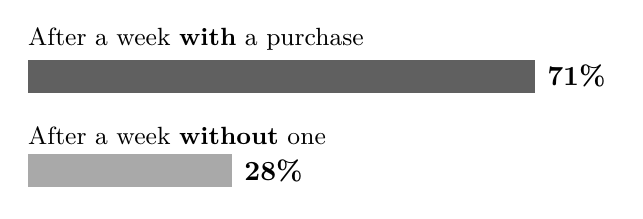
\begin{tikzpicture}[x=0.075\linewidth,y=1cm]
  \def\barh{0.42}
  \node[anchor=south west,font=\small,inner sep=0pt] at (0,1.98) {After a week \textbf{with} a purchase};
  \fill[ink!72] (0,1.45) rectangle (7.08,1.45+\barh);
  \node[anchor=west,font=\bfseries] at (7.12,1.45+\barh/2) {71\%};
  \node[anchor=south west,font=\small,inner sep=0pt] at (0,0.78) {After a week \textbf{without} one};
  \fill[bargray] (0,0.25) rectangle (2.85,0.25+\barh);
  \node[anchor=west,font=\bfseries] at (2.89,0.25+\barh/2) {28\%};
\end{tikzpicture}\par
\vspace{4pt}
{\footnotesize\color{muted}dunnhumby's public \emph{Complete Journey} data: all household-weeks of 2,500 households
over 102 weeks. Exact rates 70.8\% and 28.5\%, a gap of 42 percentage points (paper, Table~2).\par}
\end{minipage}\hfill
\begin{minipage}[t]{0.42\textwidth}
\vspace{0pt}\raggedright
{\bfseries Two questions that sound alike}\par
\vspace{7pt}
``Do customers who shop this week tend to come back next week?''\par
\vspace{1pt}{\bfseries The records answer this clearly. Yes.}\par
\vspace{9pt}
``Does a promotion make customers come back more, after it ends, than they would have
otherwise?''\par
\vspace{1pt}{\bfseries The records cannot answer this. A test with a holdout
group can.}\par
\end{minipage}

\vfill
{\footnotesize\color{muted}
Full evidence: Andreyev (2026), \emph{Heterogeneity, Latent State or Purchase History? Known-Truth
Limits on Attributing Persistence in a Household Purchase Panel}
(\href{https://github.com/rtmandreyev/shopping-persistence-reproduction/blob/main/paper/main.pdf}{PDF}).
Code, data instructions and checks:
\href{https://github.com/rtmandreyev/shopping-persistence-reproduction}{github.com/rtmandreyev/shopping-persistence-reproduction}.\par}
}

\newpage
% ============================================================================
% WHY REPEAT SHOPPING IS NOT PROOF OF LOYALTY
% ============================================================================
\section{Why repeat shopping is not proof of loyalty}

A promotion goes out. Some recipients shop that week, and many of them shop again the week
after. That sequence looks like the promotion building loyalty. The trouble is
that customers who shop in one week tend to shop in the next whether or not a promotion was
involved, and there are three ordinary explanations for why.

\vspace{6pt}
% Figure B. Three explanations that produce the same observed pattern.
% Solid arrows: what each explanation proposes. Dashed line: the association seen in data.
\begin{center}
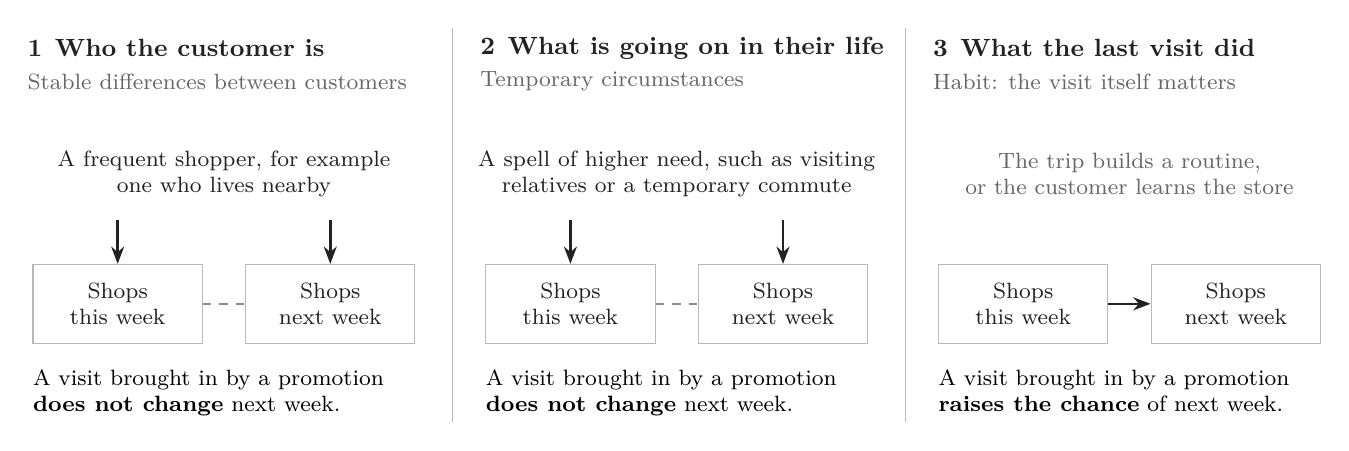
\begin{tikzpicture}[
  wk/.style={draw=rulec,fill=white,minimum width=2.15cm,minimum height=1cm,align=center,font=\footnotesize,text=ink},
  cause/.style={minimum width=4.7cm,minimum height=1.15cm,align=center,font=\footnotesize,text=ink},
  arr/.style={-{Stealth[length=2.2mm]},line width=0.9pt,color=accent},
  obs/.style={dashed,line width=0.8pt,color=faint},
  ttl/.style={font=\bfseries\small,text=ink,anchor=west,inner sep=0pt},
  sub/.style={font=\footnotesize,text=muted,anchor=west,inner sep=0pt},
  res/.style={font=\footnotesize,align=left,anchor=north west,inner sep=0pt}]
\foreach \x/\n/\t/\s in {0/1/Who the customer is/Stable differences between customers,
                         5.75/2/What is going on in their life/Temporary circumstances,
                         11.5/3/What the last visit did/Habit: the visit itself matters} {
  \node[ttl] at (\x,4.75) {\n\enspace\t};
  \node[sub] at (\x,4.32) {\s};
  \node[wk] (a\n) at (\x+1.15,1.5) {Shops\\ this week};
  \node[wk] (b\n) at (\x+3.85,1.5) {Shops\\ next week};
}
\node[cause] (c1) at (2.5,3.15) {A frequent shopper, for example\\ one who lives nearby};
\node[cause] (c2) at (8.25,3.15) {A spell of higher need, such as visiting\\ relatives or a temporary commute};
\node[font=\footnotesize,text=muted,align=center] at (14,3.15) {The trip builds a routine,\\ or the customer learns the store};
\foreach \n in {1,2} {
  \draw[arr] (c\n.south -| a\n.north) -- (a\n.north);
  \draw[arr] (c\n.south -| b\n.north) -- (b\n.north);
  \draw[obs] (a\n.east) -- (b\n.west);
  \node[res] at (a\n.south west) [yshift=-9pt] {A visit brought in by a promotion\\ \textbf{does not change} next week.};
}
\draw[arr] (a3.east) -- (b3.west);
\node[res] at (a3.south west) [yshift=-9pt] {A visit brought in by a promotion\\ \textbf{raises the chance} of next week.};
\draw[rulec] (5.4,0) -- (5.4,5.0);
\draw[rulec] (11.15,0) -- (11.15,5.0);
\end{tikzpicture}
\end{center}
\vspace{-2pt}
\note{Each panel is a possible explanation, not a finding. Solid arrows show how that explanation
would produce the pattern. The dashed line is the pattern itself: the two weeks go together
although neither visit causes the other.}

All three explanations produce the same line in a sales report: customers who shopped
recently shop again. They can also operate together. Only the third means that a visit bought
with a promotion has value beyond that visit. Under the first two explanations, bringing a customer in this
week does not by itself raise their chance of returning next week. Repeat shopping among
promoted customers is what all three predict, so it cannot tell them apart.

Targeting makes this worse. Campaigns usually go to customers who already shop often or
recently, the customers most likely to come back anyway. Comparing their return rate with
that of customers who were not targeted mixes two things: how the two groups differed to begin
with, and whatever the campaign did. Unless the rule used to choose them is recorded and taken into
account, there is no way to separate the two.

\vspace{2pt}
\begin{sidebar}{Predicting behavior is not the same as changing it}
Recent purchases are a useful input to a model that forecasts who will shop next week. In the
study, knowing which recent weeks a household shopped improved the forecast beyond knowing how
often it usually shops, though by less than knowing how often it shops in the first place. That
makes recent behavior valuable for forecasting demand and deciding whom to contact.

It does not show that creating a recent purchase, for example with a promotion, will raise the
chance of the next one. A simulated population in which past purchases had no effect at all,
and shopping followed only stable differences and circumstances that drifted from week to week,
gained just as much forecasting accuracy from recent purchases as the real data did. When
circumstances change slowly, a recent purchase is the best available sign of what they are now.
\end{sidebar}

\newpage
% ============================================================================
% WHAT THE EVIDENCE ESTABLISHES
% ============================================================================
\section{What the evidence establishes}

Section numbers refer to the research paper.

\vspace{1pt}
{\small
\renewcommand{\arraystretch}{1.14}
\begin{tabularx}{\textwidth}{@{}L{2.9cm}YL{4.4cm}@{}}
\arrayrulecolor{accent}\toprule[0.6pt]
{\color{accent}\bfseries Step} & {\color{accent}\bfseries What it found} & {\color{accent}\bfseries What it means}\\
\arrayrulecolor{rulec}\midrule
\textbf{The raw pattern}\newline\src{§2.2, Table 2} &
70.8\% of households that shopped in a week shopped the next week, against 28.5\% of those
that did not, a gap of 42 percentage points. &
Repeat shopping is strong and easy to see. \\
\midrule
\textbf{Each household compared with itself}\newline\src{§2.2, Table 2} &
Comparing each household with its own usual rate cuts the gap almost in half, to 23 points.
Also allowing for weeks when everyone shops more or less leaves 17. The exact size depends on
how it is measured, but it stays above zero in every check. &
A large part of the raw gap goes with who the customer is, though the study does not split it
into shares. Persistence remains. \\
\midrule
\textbf{Forecasting next week}\newline\src{§4, Table 3} &
Which recent weeks a household shopped improves the forecast beyond its usual rate. A
simulated population with no habit at all gains just as much. &
Recent behavior is good for forecasting. It is not evidence of habit. \\
\midrule
\textbf{The campaign records}\newline\src{§3} &
Before each of the retailer's 30 campaigns, recipients already brought it 1.6 to 3.75 times
as much revenue as non-recipients. The rule for choosing them is not recorded, and no holdout
or lottery is documented. &
The records cannot support a credible estimate of what any campaign did, in either direction. \\
\midrule
\textbf{Testing the explanations}\newline\src{§5, §6.2} &
Simulated customer populations built on each explanation were compared with the real
week-to-week pattern. Stable differences alone reproduce essentially none of it and are
rejected, under the study's main uncertainty measure, for both of the ways of describing
customer differences that were tested. Temporary circumstances and habit both remain possible.
With one of those descriptions the study's specific habit model failed to fit; with the other,
the circumstances model fit. Neither explanation was ever favored. &
Persistence beyond stable differences remains. These records do not identify its source. \\
\midrule
\textbf{Checking the method on known answers}\newline\src{§6.1, Figure 1} &
On simulated data where the answer was known, the comparison never attributed persistence to
habit when the data contained no habit effect. It also often missed habit effects that were
present. At the main setting, habit that raised next week's chance of shopping by 15 to 30 points was found in at most 65\% of
simulated datasets, and habit of 10 points or less almost never. A looser setting found about
90\% of the strongest effects, still with no false alarms, but did worse on some others. &
An unresolved result is not evidence of no habit. Habit large enough to matter commercially
could be present and go unseen. \\
\midrule
\textbf{A stress test}\newline\src{§7, Table 5} &
Simulations driven by learned decision models (see the last page) gave the same picture. Where
there was no habit, none was labeled habit. Where habit was built in a form different from the
one the method assumes, it was never detected. Most of these effects were small, and the larger
ones came from one model the paper treats as exploratory. &
No false alarms occurred, but habit of an unfamiliar form went undetected. \\
\arrayrulecolor{accent}\bottomrule[0.6pt]
\end{tabularx}
}

\vspace{4pt}
\needspace{5\baselineskip}
A large part of the raw 71\% versus 28\% gap goes with who the customer is. Under the study's
main comparison, differences between customers alone cannot account for the rest, and these
records cannot identify the source of what remains. Answering that question requires better data, from
a designed test, rather than another analysis of the same records.

\needspace{8\baselineskip}
\section{What the evidence does not establish}

\begin{itemize}[itemsep=4pt]
\item \textbf{That promotions do not work.} No campaign effect was estimated, positive or
negative. The campaign records do not allow one.
\item \textbf{That habit is absent.} The method misses most habit effects of modest size, so an
unresolved result leaves room for effects large enough to matter.
\item \textbf{That the persistence is all circumstances.} Temporary circumstances and habit both
remain possible. The comparison had no model that combines the two, and other mechanisms, such
as households stocking up, were not modeled.
\item \textbf{That the numbers carry over unchanged.} They come from one retailer and describe
whether a household shops there in a given week, not how much it spends.
\end{itemize}

% ============================================================================
% WHAT TO DO NEXT
% ============================================================================
\section{Measure the lift with a holdout group}

The question a retailer needs answered is causal: how much more do customers shop
\emph{because of} the campaign, while the offer runs and after it ends? That can be measured
directly by withholding the campaign from a randomly chosen part of the customers who would
otherwise have received it. If eligible customers are assigned to the promotion or the holdout
by a random draw, the two groups differ at the start only by chance. A difference in their
later shopping larger than chance would produce can then be attributed to the campaign. This
works for offers sent to named customers, by mail, email or app. Shelf prices, circulars and
media reach everyone and need comparisons between stores or regions instead. The design advice
here and in the next section is standard practice, not a finding of the study.

\vspace{6pt}
% Figure D. Holdout design.
\begin{center}
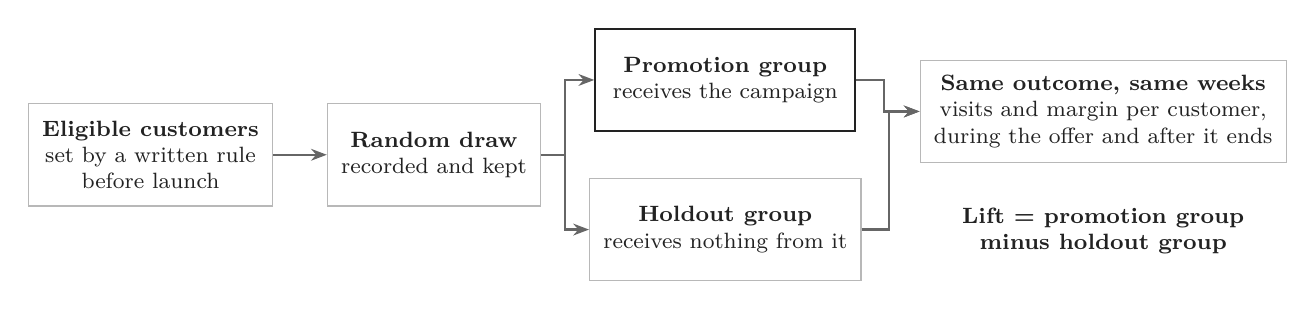
\begin{tikzpicture}[
  font=\footnotesize,
  box/.style={draw=rulec,minimum height=1.3cm,align=center,text=ink,inner sep=5pt},
  arr/.style={-{Stealth[length=2mm]},line width=0.8pt,color=muted}]
  \node[box,minimum width=3.0cm] (elig) at (0,0) {\textbf{Eligible customers}\\ set by a written rule\\ before launch};
  \node[box,minimum width=2.5cm] (rand) at (3.6,0) {\textbf{Random draw}\\ recorded and kept};
  \node[box,draw=ink,line width=0.8pt,minimum width=3.3cm] (trt) at (7.3,0.95) {\textbf{Promotion group}\\ receives the campaign};
  \node[box,minimum width=3.3cm] (hold) at (7.3,-0.95) {\textbf{Holdout group}\\ receives nothing from it};
  \node[box,minimum width=4.4cm] (meas) at (12.1,0.55) {\textbf{Same outcome, same weeks}\\ visits and margin per customer,\\ during the offer and after it ends};
  \node[font=\footnotesize\bfseries,text=accent,align=center,anchor=north] at (12.1,-0.55) {Lift = promotion group\\ minus holdout group};
  \draw[arr] (elig) -- (rand);
  \draw[arr] (rand.east) -- ++(0.3,0) |- (trt.west);
  \draw[arr] (rand.east) -- ++(0.3,0) |- (hold.west);
  \draw[arr] (trt.east) -- ++(0.35,0) |- (meas.west);
  \draw[arr] (hold.east) -- ++(0.35,0) |- (meas.west);
\end{tikzpicture}
\end{center}

\vspace{-2pt}
{\small
\renewcommand{\arraystretch}{1.2}
\begin{xltabular}{\textwidth}{@{}L{3.1cm}Y@{}}
\arrayrulecolor{accent}\toprule[0.6pt]
{\color{accent}\bfseries Decide in advance} & {\color{accent}\bfseries How, and why}\\
\arrayrulecolor{rulec}\midrule
\endhead
\textbf{Who is eligible} & Write the rule down before anyone is assigned. The measured lift
applies to customers who meet this rule, not to everyone. \\
\midrule
\textbf{How customers are assigned} & By a random draw within the eligible group, not by a
score or by judgment, and store the draw with the campaign. Drawing separately within groups of
similar past shopping, and adjusting for each customer's shopping before the campaign when the
results are analyzed, make the comparison sharper for the same number of customers. \\
\midrule
\textbf{What the holdout gets} & Nothing from this campaign. Other campaigns should treat both
groups alike. Campaigns triggered by a recent purchase will fire more often in the promotion
group, so pause them or log them. Where campaigns overlap heavily, a standing holdout kept out
of all campaigns gives the cleanest comparison. \\
\midrule
\textbf{The outcome} & Visits per customer, and ideally contribution margin per customer. Report
the weeks while the offer runs separately from the weeks after it expires. Measure the lift on
all visits; visits that redeem the campaign's own coupons can be reported but not subtracted,
since the holdout has none. If trips are recorded only when a loyalty card is scanned, check
that the share of identified trips is similar in both groups. \\
\midrule
\textbf{The window and the read-out} & The offer period plus enough later weeks to see whether
visits were only pulled forward or customers stocked up, which shows up as fewer visits later.
Fix the read-out date and do not stop early because an interim result looks good. \\
\midrule
\textbf{The size of the groups} & Large enough to tell the expected lift apart from the
break-even lift (next section), not only from zero. The analytics team can size the groups
once that target, the usual visit rate and its variability are known. \\
\arrayrulecolor{accent}\bottomrule[0.6pt]
\end{xltabular}
}

\subsection{Why the assignment record matters}
A campaign table that says only which customers received an offer is not enough. In the
study's data, campaign recipients were already more active than non-recipients before every
one of the retailer's 30 campaigns, bringing it 1.6 to 3.75 times as much revenue. For the
median campaign, 86\% of recipients were also listed for another campaign running at the same
time, and the rule used to choose recipients was not recorded. Comparing recipients with
everyone else mixes the campaign's effect with the reasons they were chosen, and nothing in the
records can separate the two. Recording eligibility and assignment at the time costs little,
and reconstructing them afterwards is usually impossible.

\subsection{What the test measures}
With random assignment, the difference between the groups measures the campaign's total effect
on eligible customers, for that offer, at that time. The lift after the offer expires is the
closest measure of the loyalty question, but it reflects everything the campaign did: any
habit, the offer's advertising effect, and visits merely moved in time. It can also be
negative, if customers stock up or learn to wait for deals. The result does not automatically
carry over to other customers, offers or seasons, and an average lift can hide differences
between groups of customers.

\vspace{1pt}
{\footnotesize\color{muted}\textbf{For analysts.}\enspace The randomized offer can also serve as
an encouragement design for the habit question itself, the effect of an induced visit on later
visits. That reading needs the further assumption that the offer affects later weeks only
through the visits it causes, which coupons valid in later weeks or the offer's advertising
effect would break. The paper cites a field experiment that used randomly assigned coupons in
this way for brand choice (Gabel, Guhl, Hitsch and Kook, 2026).\par}

% ============================================================================
% IS THE LIFT WORTH PAYING FOR?
% ============================================================================
\needspace{14\baselineskip}
\section{Deciding whether the lift pays}

A lift that is clearly above zero is not necessarily worth paying for. The campaign is worth running
if the extra contribution it creates is larger than what it costs, and that threshold can be
set before the test, from the campaign's own economics.

\vspace{1pt}
{\small
\renewcommand{\arraystretch}{1.18}
\begin{tabularx}{\textwidth}{@{}>{\centering\arraybackslash}p{0.7cm}Y@{}}
\arrayrulecolor{accent}\toprule[0.6pt]
$N$ & Customers who receive the campaign. \\
\arrayrulecolor{rulec}\midrule
$F$ & Fixed cost of the campaign: design, setup and analysis. \\
\midrule
$c$ & Variable cost per customer who receives it: delivery, plus the cost of discounts redeemed,
including discounts given to customers who would have shopped anyway. Use an expected
redemption rate before the test and the measured one after it. \\
\midrule
$m$ & Contribution margin of one extra visit, before the campaign's discount (already counted in
$c$): what the basket adds to profit after the cost of the goods and other variable costs.
Margin, not revenue. \\
\midrule
$L$ & The lift: extra visits per customer reached, caused by the campaign over the window. It is
the promotion group's average minus the holdout's, counted over the whole window, so visits that
were only pulled forward within the window cancel out. \\
\arrayrulecolor{accent}\bottomrule[0.6pt]
\end{tabularx}
}

\vspace{6pt}
\begin{formulabox}
\centering
The campaign pays if\quad
$N \times L \times m \;\ge\; F + N \times c$,\quad
so the break-even lift is\quad
$\displaystyle L^{*} = \frac{c + F/N}{m}.$\par
\vspace{5pt}\raggedright\small
In words: each customer reached must produce enough extra visits that their margin covers the
cost of reaching that customer plus that customer's share of the fixed cost.
\end{formulabox}

\begin{itemize}[itemsep=4pt]
\item \textbf{Measure per customer reached, not per redeemer.} Customers who ignore the offer
still cost something to reach, and the holdout comparison is only fair for the whole assigned
group.
\item \textbf{Prefer measured margin to an assumed one.} If the test records each customer's
margin after the campaign's discounts, the difference between the groups in that margin
replaces both $L \times m$ and the discount part of $c$. It also captures changes in basket
size and full-price purchases replaced by discounted ones.
\item \textbf{Keep the rollout decision separate from the test.} Money already spent on the test
does not count when deciding whether to roll out. Use the rollout's own fixed cost and number of
customers.
\item \textbf{Count only the weeks you can defend.} A lift claimed to last for months should be
measured for months. Over horizons longer than a few months, discount future margin.
\item \textbf{Report the lift in two parts.} The lift after the offer expires bears on
loyalty. The total lift is the investment question, and a campaign can pay for itself with no
loyalty effect at all.
\end{itemize}

\needspace{12\baselineskip}
\subsection{Compare the result with break-even, not with zero}
A test reports the lift with a range of plausible values (a confidence interval). The useful
question is where that range sits relative to the break-even lift. Statistical significance
only says whether it excludes zero. Agree in advance what each outcome will trigger.

\vspace{4pt}
% Figure E. Schematic: three possible test results against the break-even lift. No data.
\begin{center}
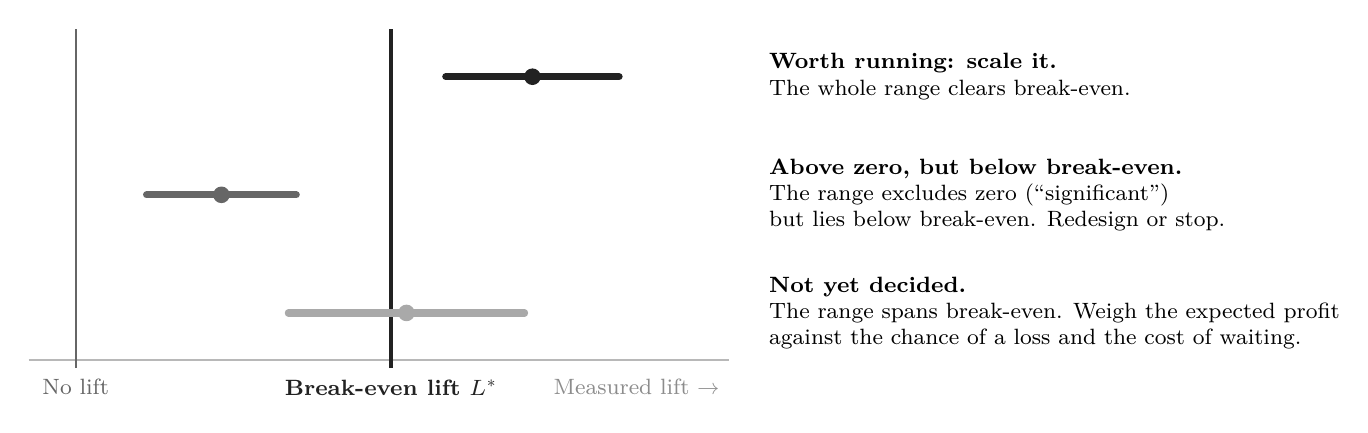
\begin{tikzpicture}[x=1cm,y=1cm,font=\footnotesize]
  \def\zx{0.6}\def\bx{4.6}
  \draw[rulec,line width=0.6pt] (0,0) -- (8.9,0);
  \draw[muted,line width=0.8pt] (\zx,-0.1) -- (\zx,4.2);
  \draw[accent,line width=1.3pt] (\bx,-0.1) -- (\bx,4.2);
  \node[anchor=north,text=muted] at (\zx,-0.12) {No lift};
  \node[anchor=north,text=accent,font=\footnotesize\bfseries] at (\bx,-0.12) {Break-even lift $L^{*}$};
  \node[anchor=north east,text=faint] at (8.9,-0.12) {Measured lift $\rightarrow$};
  \foreach \lo/\hi/\y/\c/\t in {
     5.3/7.5/3.6/accent/{\textbf{Worth running: scale it.}\\ The whole range clears break-even.},
     1.5/3.4/2.1/caution/{\textbf{Above zero, but below break-even.}\\ The range excludes zero (``significant'')\\ but lies below break-even. Redesign or stop.},
     3.3/6.3/0.6/bargray/{\textbf{Not yet decided.}\\ The range spans break-even. Weigh the expected profit\\ against the chance of a loss and the cost of waiting.}} {
    \draw[\c,line width=2.6pt,line cap=round] (\lo,\y) -- (\hi,\y);
    \fill[\c] ({(\lo+\hi)/2},\y) circle (3pt);
    \node[anchor=west,align=left,inner sep=0pt] at (9.4,\y) {\t};
  }
\end{tikzpicture}
\end{center}

\vspace{2pt}
\begin{hypo}
{\bfseries Illustration with invented numbers.}\enspace Every value here is hypothetical. None
comes from the study, and none describes any real retailer.

A campaign reaches $N = 100{,}000$ customers. The fixed cost is $F = \$50{,}000$, the variable
cost is $c = \$2$ per customer reached, and the contribution margin is $m = \$10$ per extra
visit. The break-even lift is
\[ L^{*} = \frac{\$2 + \$50{,}000 / 100{,}000}{\$10} = 0.25 \text{ extra visits per customer reached.} \]
If customers shop at most once a week, over an eight-week window that is an average gain of
about 3 percentage points in each customer's weekly chance of shopping. Suppose the test finds
0.10 extra visits per customer, with a plausible range of 0.06 to 0.14. That is the middle case
in the chart: the lift is clearly above zero, and the campaign still loses money. It creates about
$100{,}000 \times 0.10 \times \$10 = \$100{,}000$ of contribution against
$\$50{,}000 + 100{,}000 \times \$2 = \$250{,}000$ of cost.
\end{hypo}

\needspace{16\baselineskip}
% ============================================================================
% CHECKLIST, INPUTS AND ABOUT THE EVIDENCE
% ============================================================================
\section{Before crediting a campaign with loyalty}

Six questions to ask of any claim that a promotion built repeat business.

\begin{enumerate}[itemsep=5pt,leftmargin=1.6em,label={\color{accent}\bfseries\arabic*}]
\item \textbf{Who was eligible?} Is there a written rule, fixed before the campaign?
\item \textbf{How were recipients chosen?} By a recorded random draw, or by a score, a list or
someone's judgment?
\item \textbf{Is there a holdout?} Did comparable eligible customers receive nothing from the
campaign?
\item \textbf{Was the outcome fixed in advance?} Does it include the weeks after the offer
expired, which is where loyalty would show?
\item \textbf{What lift breaks even?} Was that number set from the campaign's costs and margins
before the results came in?
\item \textbf{Does the measured lift clear it?} Not just zero, but break-even.
\end{enumerate}

If the answer to the second or third question is no, repeat visits among recipients say little
about what the campaign caused.

\subsection{Inputs to gather before the test}
\vspace{3pt}
{\small
\begin{tabularx}{\textwidth}{@{}YY@{}}
\textbullet\ Margin per visit, by customer group if possible & \textbullet\ Number of eligible customers \\
\textbullet\ Delivery cost and expected redemption rate & \textbullet\ Usual weekly visit rate and how much it varies \\
\textbullet\ Fixed cost of the campaign and of a rollout & \textbullet\ Calendar of other campaigns in the same weeks \\
\textbullet\ Share of trips identified by loyalty card & \textbullet\ Who owns the read-out, and its date \\
\end{tabularx}
}

\section{About the evidence}

\textbf{The data.}\enspace \emph{The Complete Journey}, a research dataset released by
dunnhumby: every recorded purchase of 2,500 households at one grocery retailer over 711 days
(102 weeks), with records of 30 marketing campaigns. The outcome throughout is whether a
household made any purchase at the retailer in a given week. Purchases elsewhere are not
recorded.

\textbf{Checking the method.}\enspace The rules for comparing explanations were recorded before
the comparison's results were computed, though after the real data's patterns had been
examined. Before it was applied to the real data, the comparison was run on simulated datasets
in which the true explanation was known, 200 datasets per scenario. Its error rates are
conditional on calibrating those simulations to the real data, and they describe its behavior
only on simulated data like the scenarios tested.

\textbf{The stress test.}\enspace For habit of other forms than the one the method assumes,
further simulated datasets borrowed their week-to-week response from existing learned decision
models: AI systems, held at fixed versions, each asked how likely a fully synthetic household,
described in writing, was to shop next week. Household differences were recalibrated to the
real data. These models are instruments for testing the method. They are not models of
customers and say nothing about how people behave. The largest habit effects among them came
from one model whose results the paper treats as exploratory.

\textbf{Limits.}\enspace One retailer, and only the decision to shop there in a given week. The
study's main uncertainty measure does not allow for shocks shared by many households at once,
so the rejection of stable differences as the sole explanation, and the other verdicts, could
be less firm than reported (paper, §8.1).

The research paper gives the full argument, the robustness
checks and every limitation. The reproduction materials check every number in the paper
against its source and, with the data from dunnhumby, recompute the empirical results.\par
\vspace{5pt}
{\small
\href{https://github.com/rtmandreyev/shopping-persistence-reproduction/blob/main/paper/main.pdf}{Research paper (PDF)}\par
\href{https://github.com/rtmandreyev/shopping-persistence-reproduction}{github.com/rtmandreyev/shopping-persistence-reproduction}\par}

\end{document}
